\documentclass{beamer}
\usepackage[utf8]{inputenc}
\usepackage{graphicx}

\usetheme{Madrid}
\usecolortheme{default}

%------------------------------------------------------------
%This block of code defines the information to appear in the
%Title page
\title[Cloud Atlas] %optional
{Cloud Atlas}

\subtitle{An LstmEncoder for UHECR AirShowers}

\author[Gianluca Becuzzi, Lucia Papalini] % (optional)
{G. Becuzzi \and L. Papalini}

\date[July 2022] % (optional)
{July 2022}

%End of title page configuration block
%------------------------------------------------------------



%------------------------------------------------------------
%The next block of commands puts the table of contents at the 
%beginning of each section and highlights the current section:

\AtBeginSection[]
{
  \begin{frame}
    \frametitle{Table of Contents}
    \tableofcontents[currentsection]
  \end{frame}
}
%------------------------------------------------------------


\begin{document}

%The next statement creates the title page.
\frame{\titlepage}


%---------------------------------------------------------
%This block of code is for the table of contents after
%the title page
\begin{frame}
\frametitle{Table of Contents}
\tableofcontents
\end{frame}
%---------------------------------------------------------


\section{Introduction}

%---------------------------------------------------------
\begin{frame}{UHECR Airshowers}

Questo lo fa la Lush

\end{frame}

%---------------------------------------------------------


%---------------------------------------------------------
\begin{frame}{Dataset, first glance}

    The dataset is composed of $10^5$ simulated events:

    \begin{itemize}
        \item $9 x 9$ grid of detectors
        \item most intense detector at the center 
        \item 80 frames of time series ($40$ $M$Hz sampling rate)
        \item 1 frame of times of first arrival 
    \end{itemize}

    The single record shape is then $(80 + 1 , 81)$

    The \texttt{pd4ml} package splits by default in $70\%$ train $30\%$ test.

\end{frame}

%---------------------------------------------------------

\section{Preprocessing}

%---------------------------------------------------------
\begin{frame}{Split the dataset}
    Using a generator (\texttt{keras.utils.Sequence})
    \begin{itemize}
        \item inherit multiprocessing features
        \item has default callbacks
    \end{itemize}
    The dataset is splitted \emph{record by record} for index shuffling

    The effect of the high reading time from memory ($\approx 3 m$s) is mitigated
    by \texttt{keras} multiprocessing
    
    For the design of the net it is convenient using \texttt{numpy} structured arrays
\end{frame}

%---------------------------------------------------------
\begin{frame}{Split the dataset: \texttt{funky\_dtype}}

    Data is extracted: from a conceptually \emph{ihomogeneous} list 
    (activity time series together with times of arrival) to
    $(80 + 1, 81) \rightarrow [("toa", (9, 9, 1)), ("timeseries", (80, 9,9))]$

    Data can be accessed depending on what is needed

\end{frame}


%---------------------------------------------------------
\begin{frame}{DataFeeder class}
    Ensures an easy way to train the subnets separately

    \begin{itemize}
        \item shuffles data randomly
        \item input fields can be specified
        \item can be extended to more complex training strategies
    \end{itemize}
    
\end{frame}

%---------------------------------------------------------
\begin{frame}{DataFeeder class}{Curriculum learning}

    Using a pre-trained network data can be ``scored'' in ascending order of difficulty

    (work in progress) This can lead to a learning speed-up and improvements in resolution
    
    Caveat: this training strategy is not well suited (conceptually at least) for regression tasks, 
    since it is not clear what a ``difficult'' sample would look like.
\end{frame}

%---------------------------------------------------------
\begin{frame}{Data Augmentation}
    Dataset has a lack of high events ($X > 850$m) so the network resolution is worse
    for samples corresponding to this range

    \begin{block}{Strategy}
        Increase the number of samples conditionally on event heigth using the
        symmetries of the problem
    \end{block}

    Data is augmented using
    \begin{itemize}
        \item flip up-down
        \item flip left right
        \item rotation of $90^{\circ}$ (x4)
    \end{itemize}
    
    It must me higlighted that only a subset of the available data undergoes this procedure.

    Augmenting the whole dataset would leave the sample distribution unchanged and thus would not lead 
    to improvements.
\end{frame}

\begin{frame}{Resolution}

    The reference article suggests using the resolution:
    \begin{block}{resolution}
        defined as the standard deviation of the distribution given by the difference between the predictions and the actual values of $X_{max}$
    \end{block}

    We point out that 
    \[\sigma^2 = \frac{1}{N}\sum_i (\delta_i - \bar{\delta})^2\]
    is a sensible estimator of ``how much the net has gone wrong'' only if $\bar{\delta} = 0$, for which the adopted resolution is equal 
    to the $RMSE$ of the distribution
    \[ RMSE^2 = \frac{1}{N}\sum_i(x_i - \hat{x}_i)^2 \]
    Since (on a typical train) $\bar{\delta} \approx 10$m we preferred the RMSE.
\end{frame}



\section{Neural Network building}

    \centering
    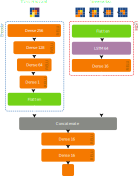
\includegraphics[width=0.6\textwidth]{model.pdf}
%---------------------------------------------------------
\begin{frame}{Overview on the network}
    The assumption that lead to this design is that from the time of arrival matrix
    it is possible to infer some kind of ``homogeneous'' shower parameters (incidence angle, spread, etc.)
    while the time series can be processed by a recurrent network.
\end{frame}

%---------------------------------------------------------
\begin{frame}{Encoder for time of arrivals}

    \includegraphics[width=\textwidth]{ENC_history.png}
    
\end{frame}


%---------------------------------------------------------
\begin{frame}{LSTM}
si spiega che cos'è
    
\end{frame}

%---------------------------------------------------------
\begin{frame}{LSTM for the time series}
    \includegraphics[width=\textwidth]{LSTM_history.png}    
\end{frame}

\begin{frame}{Subnets performance}
    \includegraphics[width=\textwidth]{sub_net_train.pdf}
\end{frame}

%---------------------------------------------------------
\begin{frame}{Concatente + dense layers}

    
\end{frame}


\begin{frame}{Subnets train freezing}
    \includegraphics[width=.8\linewidth]{freezetraining_2.pdf}
\end{frame}

\begin{frame}{Subnets train freezing}
    \includegraphics[width=.8\linewidth]{freezetraining.pdf}
\end{frame}

%---------------------------------------------------------
\begin{frame}{Network's output}

    
\end{frame}

%---------------------------------------------------------
\begin{frame}{Hyperparameters tuning}

    
\end{frame}


%---------------------------------------------------------
\begin{frame}{Whole Network performance}

    
\end{frame}

\begin{frame}{Test setup on CircleCI}

    
\end{frame}

%---------------------------------------------------------
\begin{frame}{Danke e bibliography}
\centering
Danke Schon

    
\end{frame}




\end{document}
